% Remplacement local des encadrés de placeholders du chapitre Brise-glace par
% les illustrations réelles. Ce fichier est chargé dans un groupe LaTeX dédié
% afin de ne pas modifier le comportement de \fbox dans le reste du dossier.
\newcounter{briseglacefigureplaceholder}
\setcounter{briseglacefigureplaceholder}{0}

\renewcommand{\fbox}[1]{%
  \stepcounter{briseglacefigureplaceholder}%
  \ifcase\value{briseglacefigureplaceholder}%
  \or
    % Déroulement général d'une partie.
    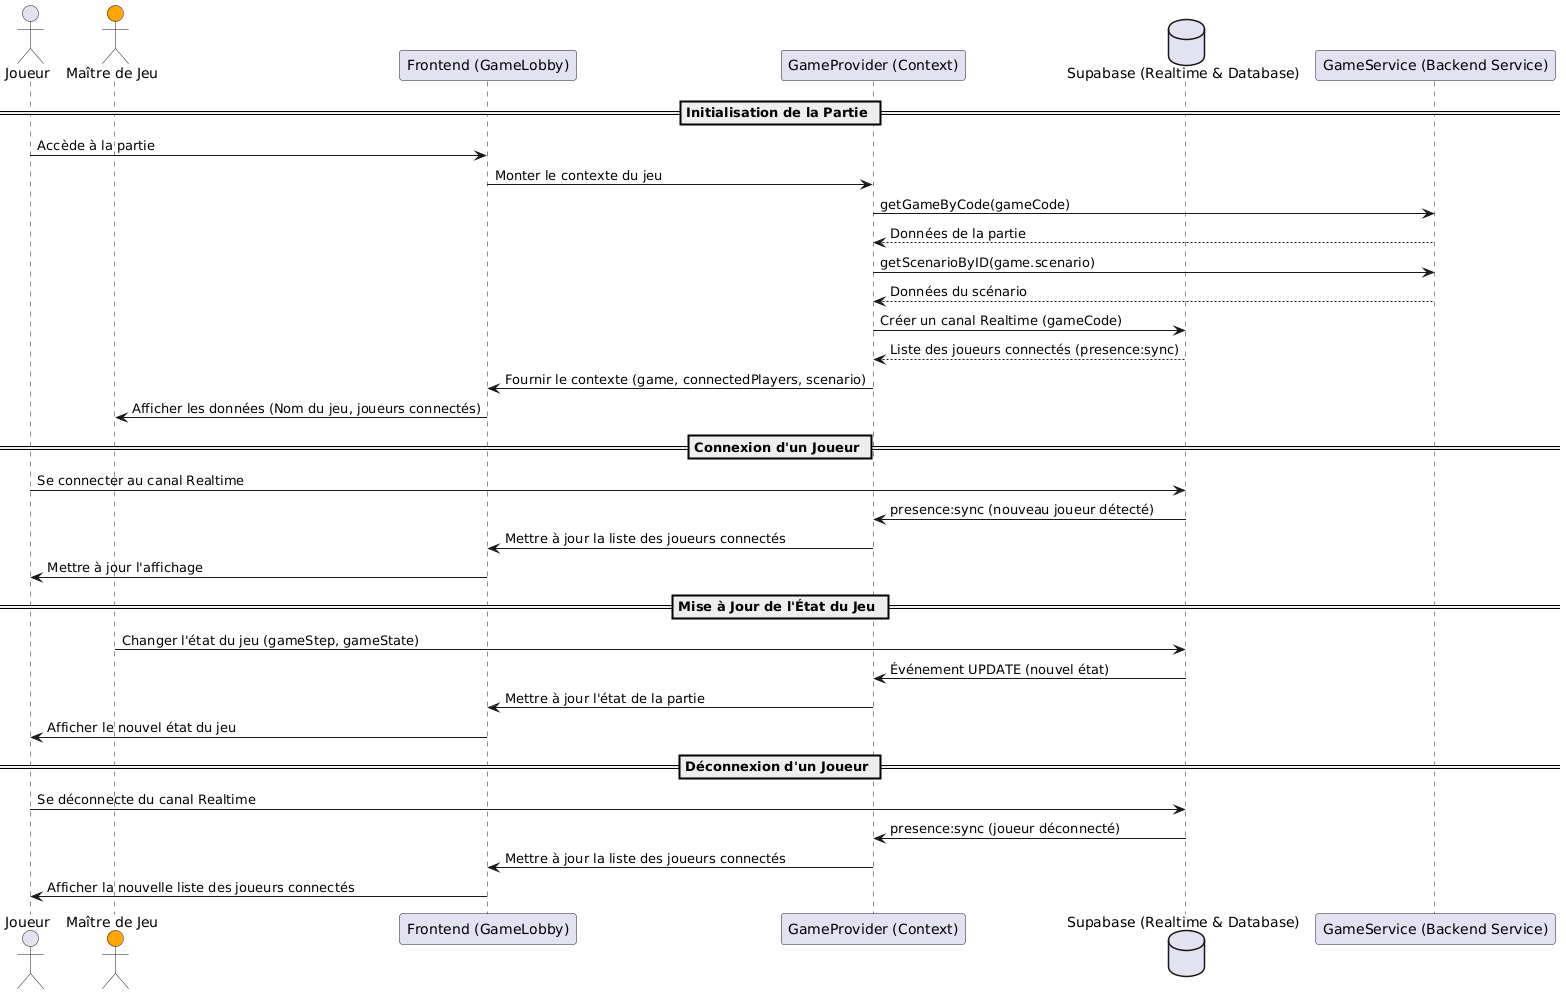
\includegraphics[width=\textwidth,height=0.48\textheight,keepaspectratio]{figures/brise_glace/sequence_partie.png}%
  \or
    % Architecture React / Supabase.
    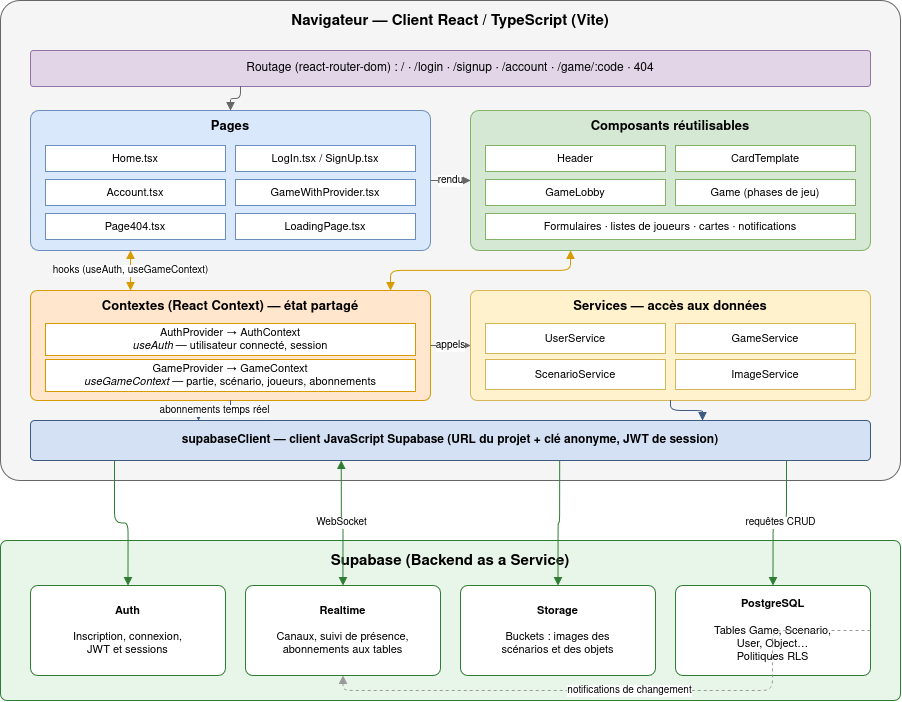
\includegraphics[width=\textwidth,height=0.52\textheight,keepaspectratio]{figures/brise_glace/architecture.png}%
  \or
    % Planche des principaux écrans. La capture du plateau provient de
    % l'application de test utilisée pour valider l'interaction de classement :
    % aucune capture du plateau final n'a été conservée.
    \begin{minipage}{\textwidth}
      \centering
      \begin{minipage}[t]{0.68\textwidth}
        \centering
        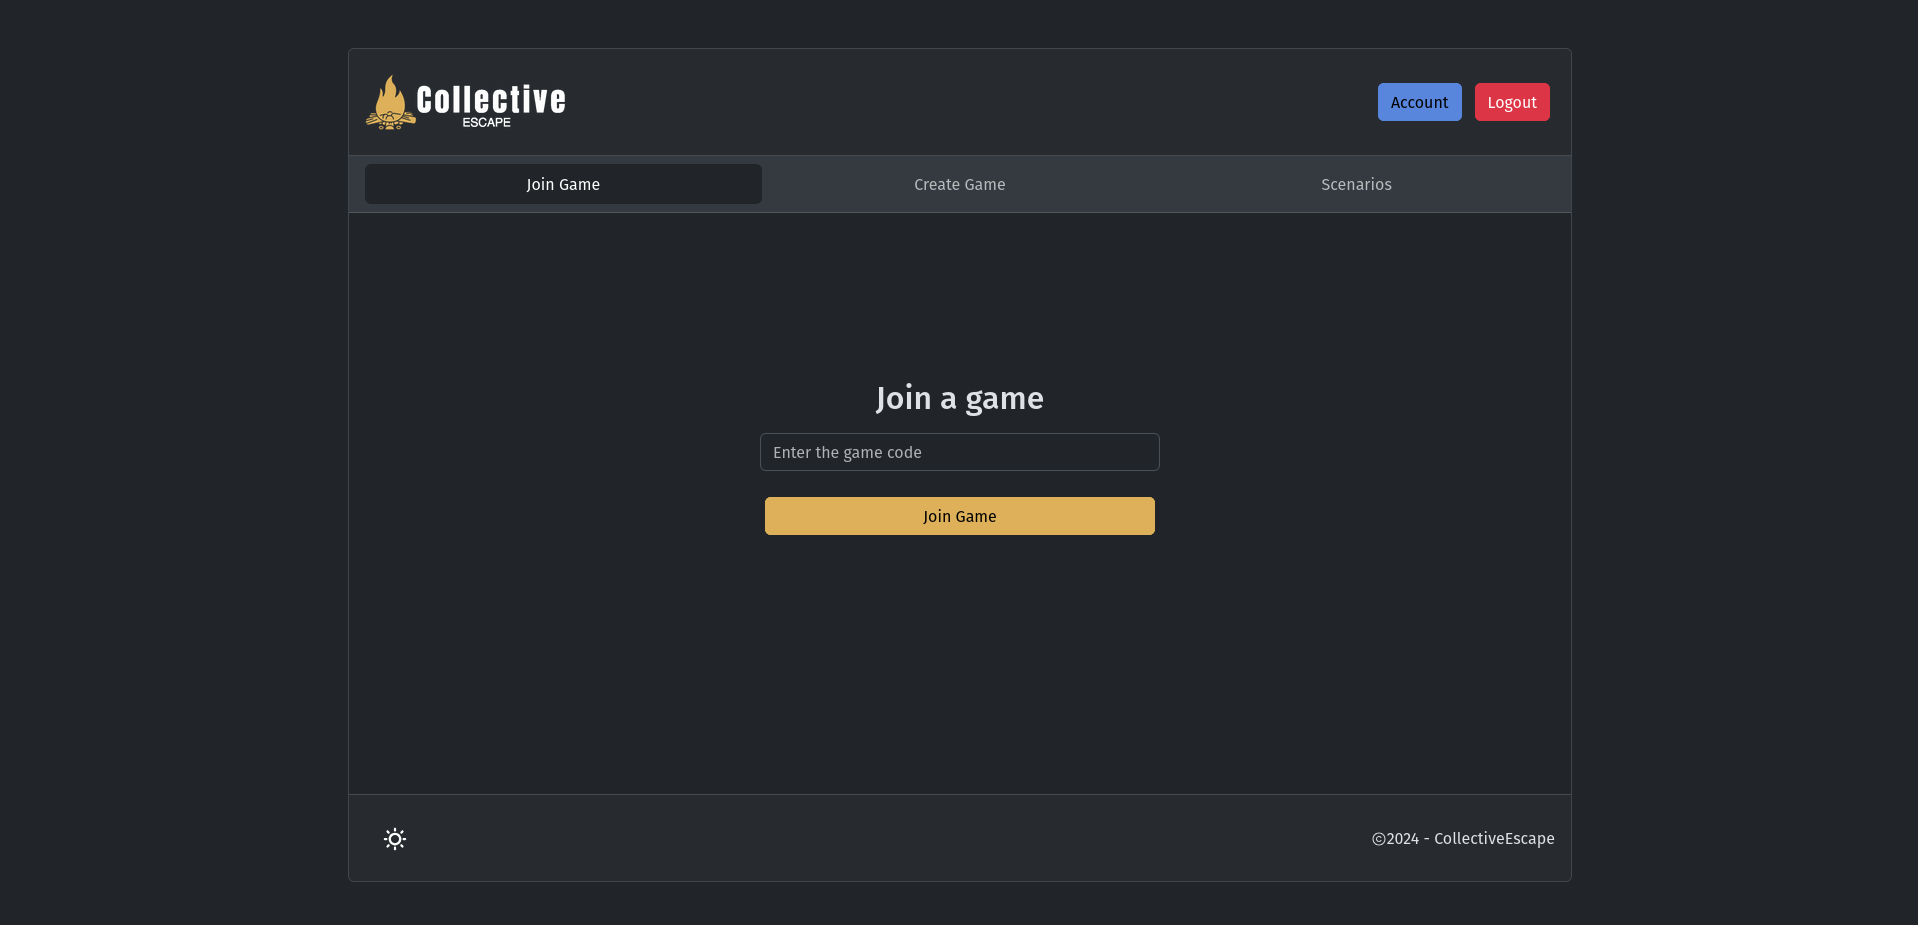
\includegraphics[width=\textwidth,height=0.17\textheight,keepaspectratio]{figures/brise_glace/home_desktop.png}\\[-0.05cm]
        {\footnotesize (a) Accueil sur ordinateur}
      \end{minipage}%
      \hfill
      \begin{minipage}[t]{0.27\textwidth}
        \centering
        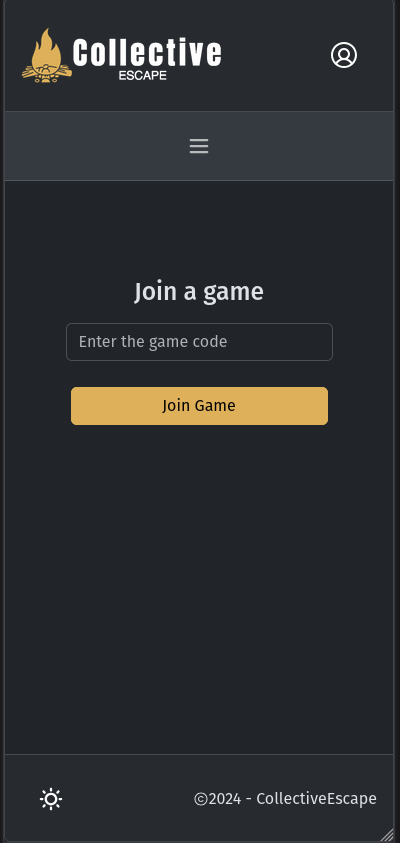
\includegraphics[width=\textwidth,height=0.17\textheight,keepaspectratio]{figures/brise_glace/home_mobile.png}\\[-0.05cm]
        {\footnotesize (b) Accueil sur mobile}
      \end{minipage}

      \vspace{0.25cm}

      \begin{minipage}[t]{0.48\textwidth}
        \centering
        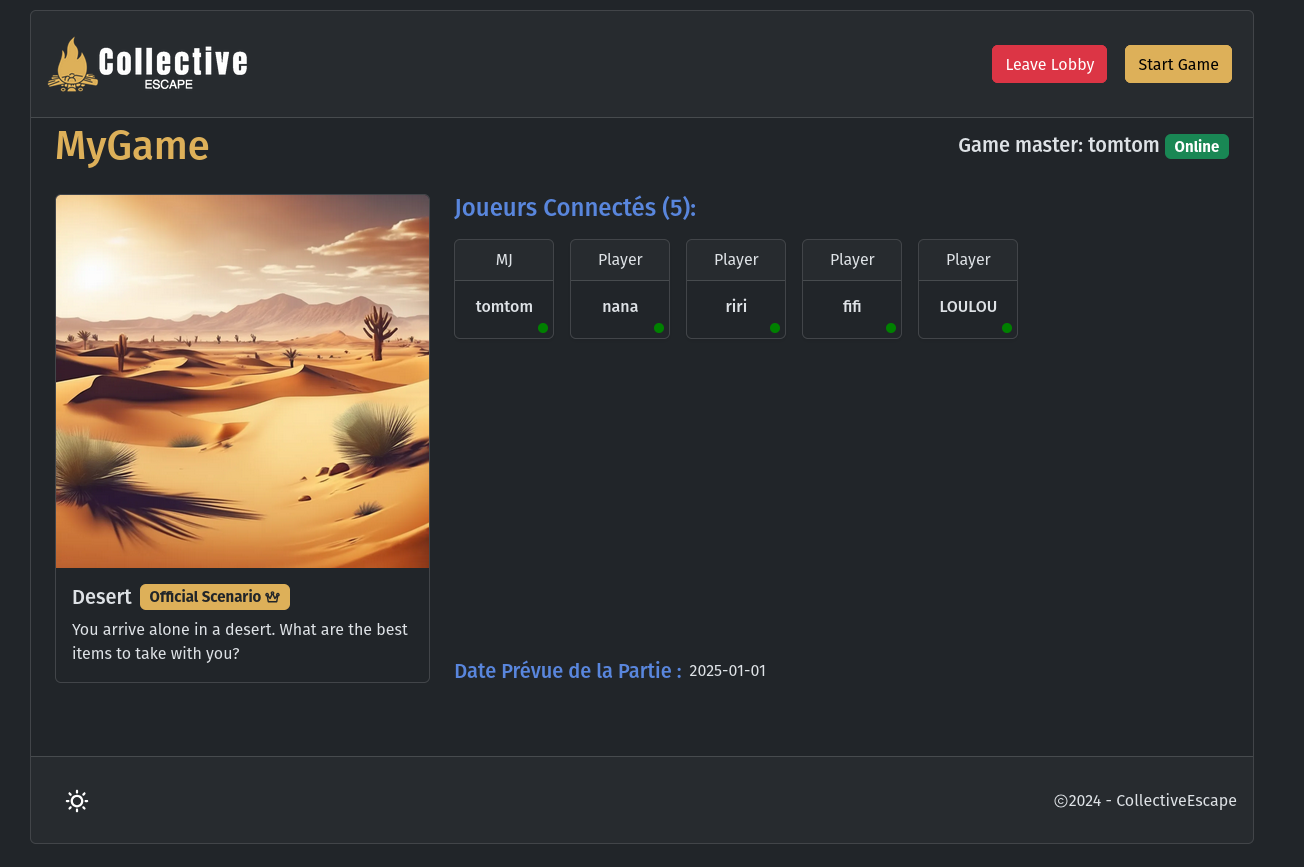
\includegraphics[width=\textwidth,height=0.18\textheight,keepaspectratio]{figures/brise_glace/lobby.png}\\[-0.05cm]
        {\footnotesize (c) Lobby d'une partie}
      \end{minipage}%
      \hfill
      \begin{minipage}[t]{0.48\textwidth}
        \centering
        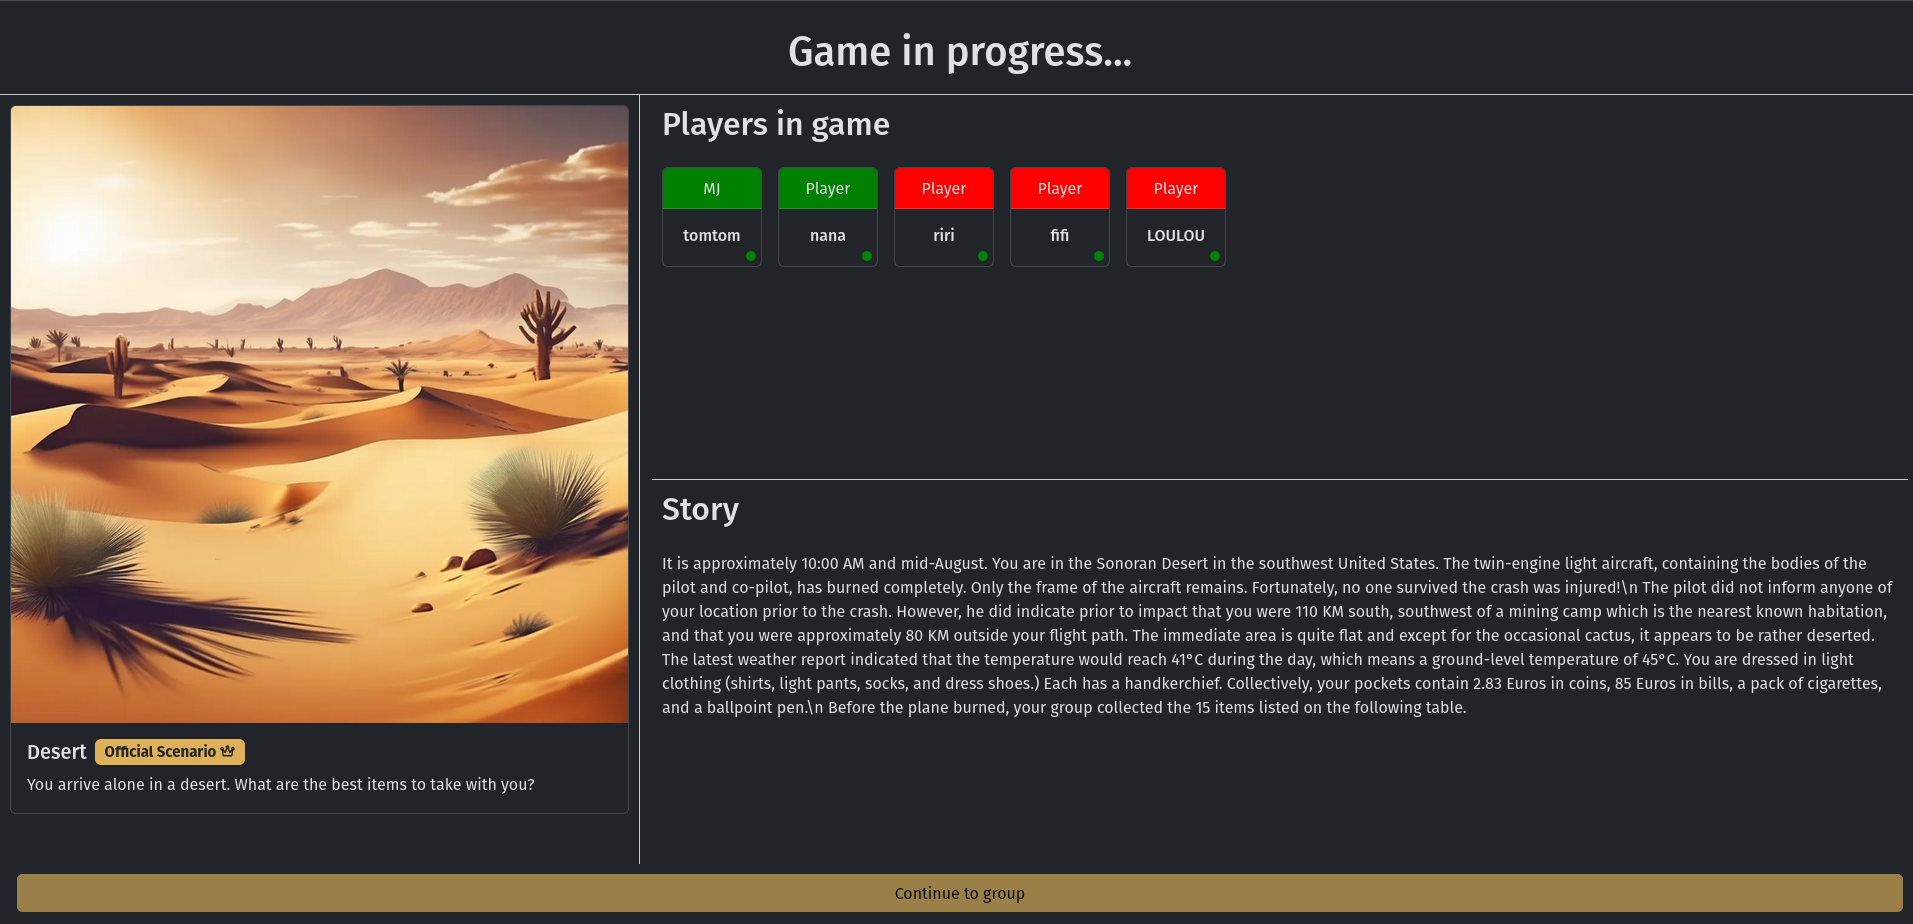
\includegraphics[width=\textwidth,height=0.18\textheight,keepaspectratio]{figures/brise_glace/ecran_game_master.png}\\[-0.05cm]
        {\footnotesize (d) Écran du maître du jeu}
      \end{minipage}

      \vspace{0.25cm}

      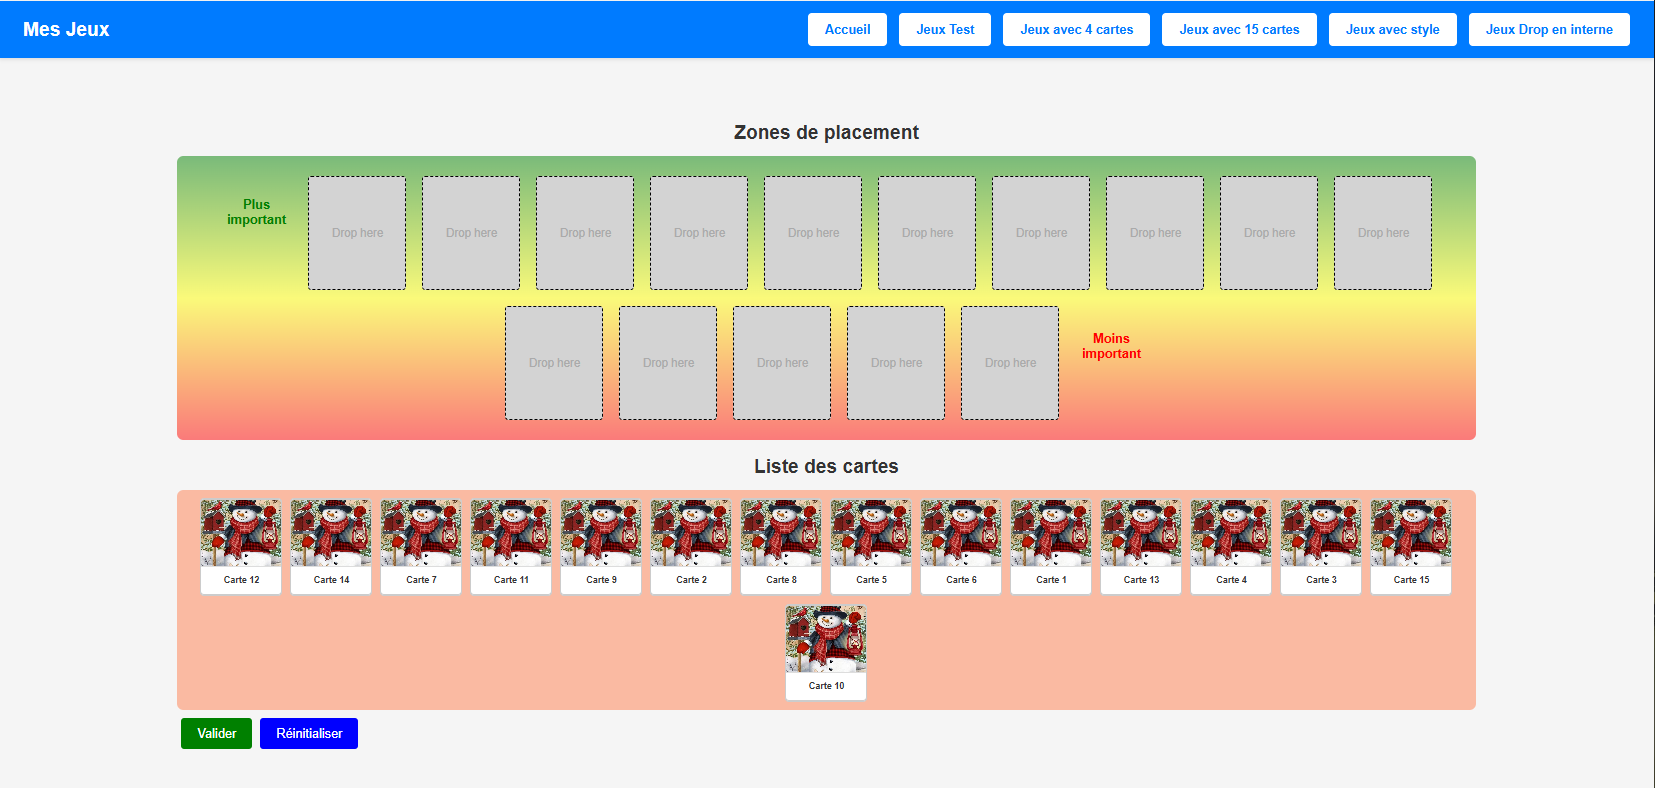
\includegraphics[width=0.82\textwidth,height=0.23\textheight,keepaspectratio]{figures/brise_glace/plateau_maquette.png}\\[-0.05cm]
      {\footnotesize (e) Plateau de l'application de test utilisée pour valider le classement (capture non finale)}\\[0.12cm]
      {\footnotesize\itshape La capture du plateau final n'ayant pas été conservée, cette illustration documente honnêtement l'état de test de l'interaction par glisser-déposer.}
    \end{minipage}%
  \else
    \PackageError{brise-glace-figures}{Nombre de placeholders Brise-glace inattendu}{Le chapitre Brise-glace contient plus de 3 appels a \string\fbox.}%
  \fi
}
